% Asset ID: A22ProjectilesTikZ-004
% Purpose: Vector projectile diagram with position and velocity components.
\documentclass[tikz,border=8pt]{standalone}
\usepackage{amsmath}
\usetikzlibrary{arrows.meta,calc}
\begin{document}
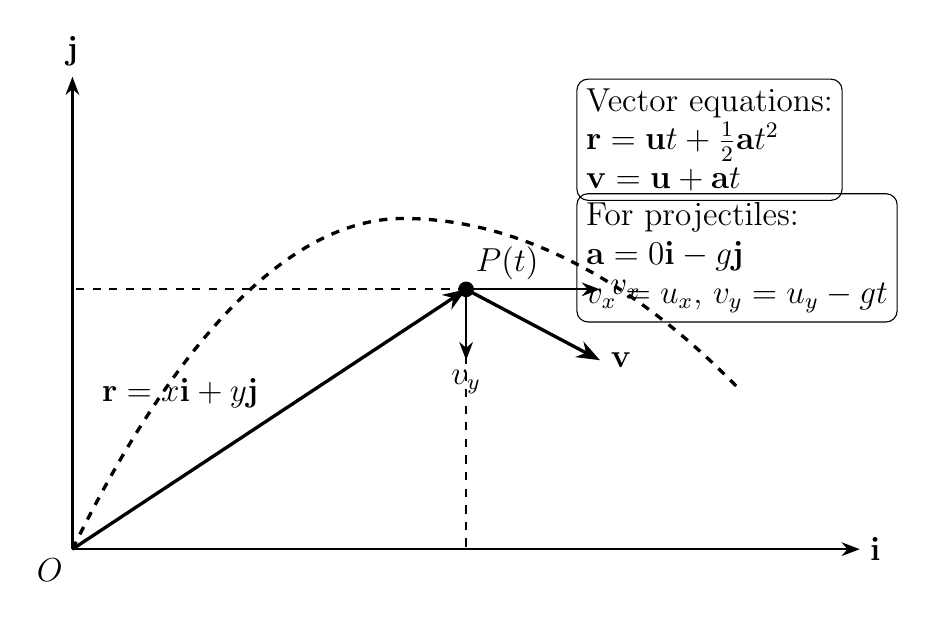
\begin{tikzpicture}[>=Stealth,axis/.style={->,thick},pathcurve/.style={dashed,very thick},vector/.style={->,very thick},comp/.style={->,thick},guide/.style={dashed,thick},label/.style={font=\large},point/.style={circle,fill=black,inner sep=2pt}]
\draw[axis] (0,0)--(10,0) node[right,label] {$\mathbf{i}$}; \draw[axis] (0,0)--(0,6) node[above,label] {$\mathbf{j}$}; \node[below left,label] at (0,0) {$O$};
\draw[pathcurve] (0,0) parabola bend (4.2,4.2) (8.5,2.0);
\coordinate (P) at (5.0,3.3); \node[point] at (P) {}; \node[above right,label] at (P) {$P(t)$};
\draw[vector] (0,0)--(P) node[midway,above left,label] {$\mathbf{r}=x\mathbf{i}+y\mathbf{j}$};
\draw[guide] (P)--(5.0,0); \draw[guide] (P)--(0,3.3);
\draw[comp] (P)--++(1.7,0) node[right,label] {$v_x$}; \draw[comp] (P)--++(0,-0.9) node[below,label] {$v_y$}; \draw[vector] (P)--++(1.7,-0.9) node[right,label] {$\mathbf{v}$};
\node[draw,rounded corners,align=left,font=\large,anchor=west] at (6.4,5.2) {Vector equations:\\$\mathbf{r}=\mathbf{u}t+\frac12\mathbf{a}t^2$\\$\mathbf{v}=\mathbf{u}+\mathbf{a}t$};
\node[draw,rounded corners,align=left,font=\large,anchor=west] at (6.4,3.7) {For projectiles:\\$\mathbf{a}=0\mathbf{i}-g\mathbf{j}$\\$v_x=u_x$, $v_y=u_y-gt$};
\end{tikzpicture}
\end{document}
